\chapter{A PX Model for Rehabilitation Exergames}
\label{ch:model}
% A model that integrates constraints, aspects, instruments and methods, evaluators and game user researchers will benefit having a model that allows understanding dimensions (ayers and time) and elements that model PX in rehabilitation exergames
As presented in \autoref{sec:ox_ux_models}, there are models to study \ac{PX} and \ac{UX}. However, those models are not sufficient to study rehabilitation exergames since these do not consider the constraints presented in \autoref{ch:characterising} and the aspects, methods and instruments presented in \autoref{ch:aspects}.

In this chapter, we present a model for studying \ac{PX} in rehabilitation exergame. It that integrates existing research with the findings presented in this document will allow studying rehabilitation exergames properly. The model allows studying existing \ac{PX} aspects and the new aspects that we have identified. Also, it will integrate rehabilitation exergames constraints into its components. First, \autoref{sec:related_work_model} presents the \ac{PX} models that we studied to build our model. Then, \autoref{sec:mats_mets_model} describes the methods that we employed to design the model. After that, \autoref{sec:findings_model} describes the proposed model. Finally, \autoref{sec:discussion_model} discusses the findings of the conducted study and \autoref{sec:conclusion_model} concludes the chapter.

% -----------------------------------------------
\section{Related work} % Related work %-----------------------------------------------
\label{sec:related_work_model}
The purpose of this study is to design a model to study \ac{PX} in rehabilitation exergames. We have identified some constraints \autoref{ch:characterising} and aspects \autoref{ch:aspects} of rehabilitation exergames from the field of physiotherapy. To design a comprehensive model we need to integrate those findings into current \ac{PX} models. Thus, this section presents the models that we considered to design our model.

We presented two models that we consider for our proposal in \autoref{sec:ox_ux_models}. First, the \ac{IMP} model \autocite{Elson2014}, which describes \ac{PX} considering three elements, player, context and game. Also, the model suggests that \ac{PX} should be studied before, during and after interaction with a game occurs. Second, the Contextual Gameplay Experience Model \autocite{Engl2013}, which considers three elements similar to those of the \ac{IMP} model and is based on \autocite{Nackea2,Nacked}; i.e., game system, player and contextual influences. In this model, those elements are layers of abstraction, in which contextual influences is the most abstract layer and the game system is the most concrete one. It also suggests that \ac{PX} occurs before, during and after interaction occurs. Below, we present the other models that we use as a base to design our model.

\subsection{A PX Framework}
\textcite{Nackea2} present a \ac{PX} framework based on three layers of abstraction: the context, the player and the game system (See \autoref{fig:px_framework}). Context is the most abstract layer. It comprises the experience resulting from interacting with other players, games and technologies over a certain time. It involves the game community and its generated knowledge. The player layer represents the experience that influences and is influenced by the actions of players. The most concrete layer is the game system and comprises perceivable and technical experience generated by games.

The model presents interrelations among the layers. The context layer shapes players' perceptions of games, e.g., through a bad review. Meanwhile, the player the layer influences the context by generating knowledge about the game. Also, players provide content and data to shape game behaviour and adjust it to their preferences. Finally, the game system layer influences players' experience through its functionality and mechanics.

Finally, the model describes how each layer is affected by time. First, the game system layer is affected by technological changes. Second, the player layer evolves due to psychological and physiological changes. Finally, the context layer changes due to social, political or economic influences.

\begin{figure}[bth]
\myfloatalign
{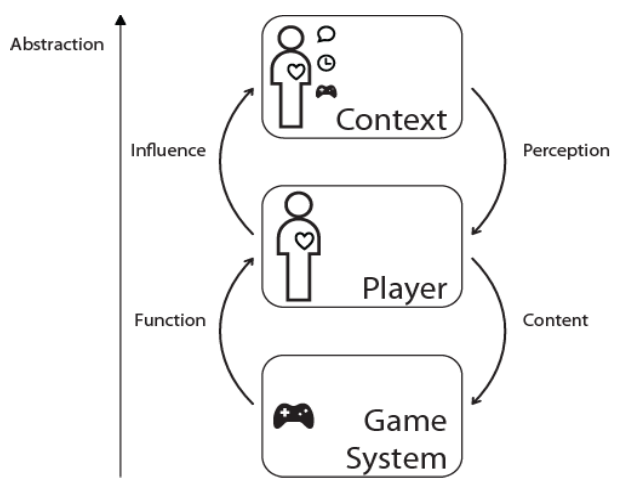
\includegraphics[width=.6\linewidth]{gfx/model/px_framework}} \quad
\caption[The PX Framework]{The \ac{PX} Framework \autocite{Nackea2}}\label{fig:px_framework}
\end{figure}

\subsection{The Game Usability Model}
\textcite{Nacked} presents the Game Usability Model that integrates \ac{PX} research into a single framework. It comprises nine entities that go from theoretical to practical and from concrete to abstract (See \autoref{fig:game_usa_model}). Three of those entities are theoretical constructs that affect \ac{PX}; i.e., technology, player and community. The technology entity is measured by the system quality and analysed using quality assurance. The player entity is measured by gameplay quality and studied using user experience analysis. Finally, the community construct is measured by the social quality and analysed using sociological studies.

This model intends to address three challenges that result when analysing \ac{PX}. The first challenge relates to \ac{PX} optimisation. According to the author, the interface of a game has to optimise \ac{PX} usability and functionality. The second challenge is the complexity of digital games, which are complex software programs due to content, controls, customisation and game design among others. The last challenge relates to time. \ac{PX} should be studied before, during and after interaction occurs. Before interaction, the state of the players and game marketing shape \ac{PX}. Also, the impact of an interaction on a player will affect preceding interactions.

\begin{figure}[bth]
\myfloatalign
{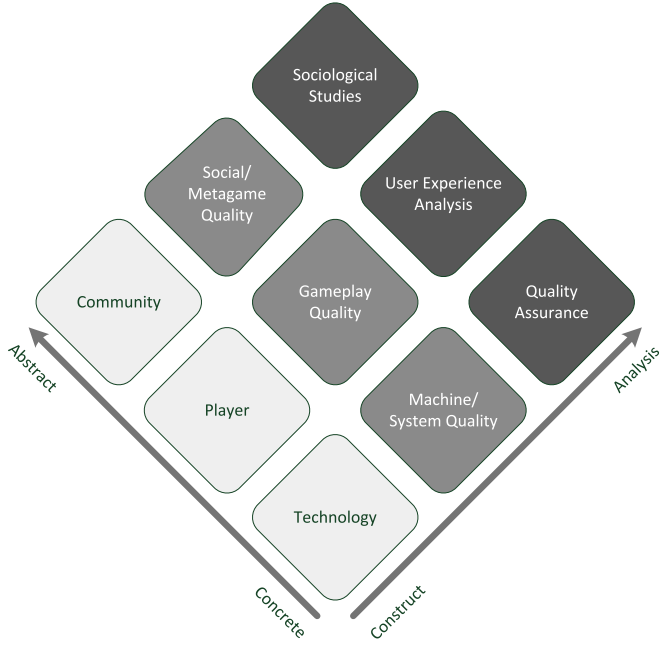
\includegraphics[width=.6\linewidth]{gfx/model/game_usa_model}} \quad
\caption[The Game Usability Model]{The Game Usability Model \autocite{Nacked}}\label{fig:game_usa_model}
\end{figure}

\subsection{The Game Experience Model}
\textcite{Fernandez2008} presents the Game Experience Model which suggests that the main result of game experience is fun. The model is based on three stages. First, the antecedents stage intends to capture the elements that motivate players to play a game, and lead to certain behaviours during an interaction. Second, the processing stage refers to the interaction moment between a player and a game. This stage depends on the players' motivation to play. Third, fun depends on the consequences of interacting with a game. These consequences can be cognitive such as thoughts and inferences, or emotional such as feelings.

The antecedents comprise players' demographics and game activity; i.e., previous experiences, game and hardware preferences and purpose. Those elements affect the motivation of players to start or continue playing a game. . 

Players' motivation determines the degree of attention and effort that they invest in a game during processing. According to the author, motivation also determines if players play using a serious or playful strategy. Additionally, games have pragmatic and hedonic attributes that affect \ac{PX}. Pragmatic attributes are assessed through the game interface and usability while hedonic attributes comprise the game mechanics (universe), the game features that trigger interactivity and the technology.

In \autocite{Fernandez}, the author conducted a study to prove the relations among the different elements of its model. The results showed that the years playing games and game genre preference define the user profile and purpose. Also, the author found that the user profile is related to motivation, but does not explain it. Furthermore, the results showed that when players are motivated, they can overcome usability shortcomings. Finally, the author found that high-quality technology and usability lead to universe appreciation.

\subsection{The Contextual Game Experience Model}
\textcite{Mayra} describes a model that considers the socio-cultural context of \ac{PX}. The author argues that games are played not only to experience fun, but also to facilitate social situations; e.g., when used to maintain or strengthen social relations. According to this model, the game experience is pre-defined, modified and post-defined by multiple dimensions. It relates to the immediate personal and social contexts.  Thus, knowing players motivations, game habits and historical reasons to play is important to understand \ac{PX}. Additionally, the contexts for digital game production, the contexts provided by earlier forms for play (i.e., people's game literacy) and the context of social norms and values influence each other and shape game experience.

\subsection{People, Places and Play Research Framework}
\textcite{DeKort2007b} present a research framework that explores game experience as a situated experience formed by co-players, audience and spatial organisation. That is, the game experience is influenced by social contexts. The model is based on the evidence that people have better experiences when playing with or against players since social settings empower or diminish emotions. The social context of gaming comprises the presence of others, their ability to monitor and communicate with players, their role in the system (i.e., co-players or audience) and their relationships.

%-----------------------------------
%\section{Aim of the study} % Aim of the study -----------------------------------

%-----------------------------------
\section{Materials and methods} % Materials -----------------------------------
\label{sec:mats_mets_model}
%% Examples: https://pdfs.semanticscholar.org/2b2f/444cb600101f8d78508b4945123938f06a0e.pdf
%% USed approach: http://eprints.uwe.ac.uk/11735/2/thematic_analysis_revised...
% Participants - Procedure
We conducted a literature review to identify existing \ac{PX} models in the Scopus database. We included models that serve to study \ac{PX}, game experience or gameplay experience. We reviewed 7 documents which were presented above (See \autoref{sec:related_work_model}). Four relevant documents were identified in Scopus, and the remaining were extracted from their references. The objective of this review was to identify common \ac{PX} constructs, dimensions and concepts of the models. Also, we use the findings of a study presented previously (See \autoref{ch:characterising}). We use both results as the source to propose a model of \ac{PX} for rehabilitation exergames.

% Analysis
We analysed data using a 'theory-driven' thematic analysis \autocite{Braun} since we had already identified a target data; i.e., \ac{PX} constructs, dimensions and concepts. First, we read the documents carefully to identify meaningful data relevant to the research aim. Each data was registered in a list including a reference to its source document. Then, we generate initial codes for each data. After that, we reviewed and grouped the codes to identify potential themes. After that, we reviewed the themes iteratively until the final themes were defined. The thematic analysis resulted in 46 initial codes grouped into the two themes.

%-----------------------------------
\section{Findings} % Findings -----------------------------------
\label{sec:findings_model}
After conducting a thematic analysis of the data collected from the documents and the results from the previous study, 46 initial codes were identified. These codes were iteratively grouped into themes until achieving a total of two main themes. The first theme is \textit{layers of abstraction} which represent the main actors that may influence \ac{PX} model. The second theme is \textit{dimensions}, which relates to the point of view or analysis in which the constructs can be understood and studied. 
%The third theme is aspects, which represents the main \ac{PX} aspects identified in the documents and the previous study. The final theme is \textit{\ac{PX} concept}, which represent the definitions and characteristics to understand the concept of \ac{PX}.

\subsection{Layers of abstraction}
\label{sec:layers_abstraction}
The study allowed to identify three main constructs of \ac{PX}. The context, the player and the game system. Those are illustrated in \autoref{fig:layersOfAbstraction} and detailed below.

\begin{figure}[bth]
\myfloatalign
{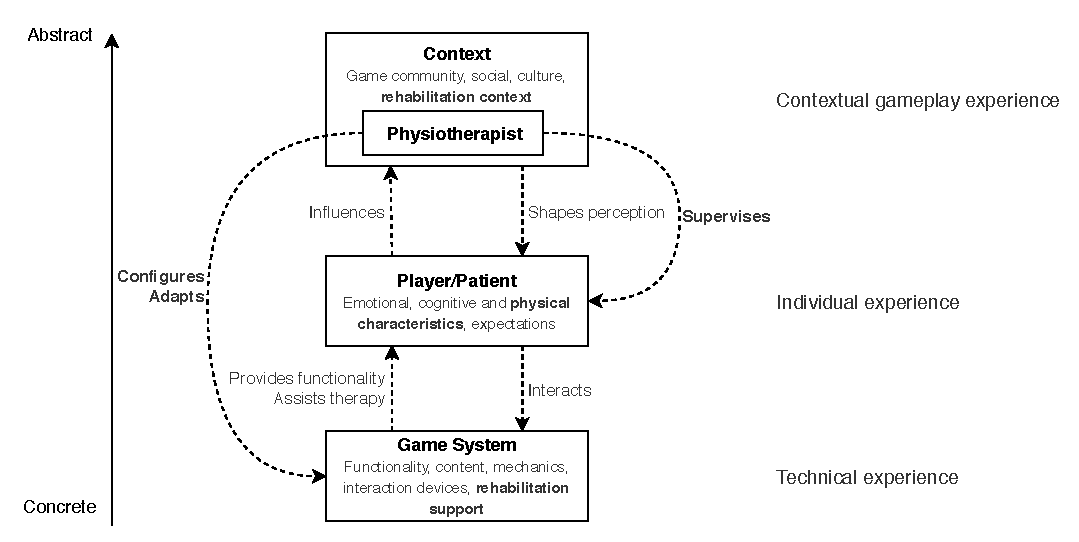
\includegraphics[width=\linewidth]{gfx/model/layersOfAbstraction}} \quad
\caption{\ac{PX} Layers of Abstraction}\label{fig:layersOfAbstraction}
\end{figure}

The \textit{Context} shapes the experience of players by means of game communities \autocite{Nacked,Nackea2,Elson2014}, other players \autocite{Nacked,Nackea2,Nackea,DeKort2007b,Elson2014}, audience \autocite{DeKort2007b,Mayra,Nackea2}, values and norms \autocite{Elson2014,Mayra}, location \autocite{Engl2013,Elson2014}, time \autocite{Engl2013}, game market \autocite{Elson2014,Nackea}, physiotherapists and rehabilitation context constraints presented in \autoref{sec:reh_context_constraints}. The context alter players' perceptions \autocite{Nackea2,Nackea}, behaviours and experiences \autocite{Engl2013}.

The \textit{Player} represents the individual experience of a person who interacts with the game system. In the case of rehabilitation exergames, a player is also a patient. It involves characteristics \autocite{Elson2014,Fernandez2008,Mayra} and psychological \autocite{Elson2014} and physiological behaviours experienced by a player. It also involves the expectations of players/patients towards their therapy. It comprises the patients' related constraints presented in \autoref{sec:reh_patients_constraints}. The \ac{PX} quality is assessed using aspects related to psychological and physiological characteristics of players.

The \textit{Game System} represents the perceivable and technical experience \autocite{Nackea2,Elson2014}. In involves content \autocite{Elson2014,Nackea2,Fernandez2008}, functionality \autocite{Engl2013,Nacked} and technology \autocite{Engl2013,Fernandez2008} of a game. Studying the game system in \ac{PX} is important since a game is a complex software system \autocite{Mayra,Nackea} and its design impacts directly on the experience that a player may have. The game system comprises the components that support a rehabilitation therapy. It involves the interaction devices constraints presented in \autoref{sec:interation_dev_constraints}. And the constraints presented in \autoref{sec:reh_goal_constraints} that impose requirements to the game system. That includes patients' safety assurance, feedback provision about progress and exercise correctness, movement mapping correctness and play time. The game system quality is assessed through playability \autocite{Engl2013,Nackea2}.

\subsection{Dimensions}
The thematic analysis allowed to identify two dimensions to study \ac{PX}, the layer of abstraction and time. The layers of abstraction represent the actors that influence \ac{PX} \autocite{Nacked,Nackea2,Engl2013,Elson2014}. There are three layers of abstraction, which are game system, player and context. The time dimension allows studying \ac{PX} before (\textit{antecedents}), during (interaction) and after (\textit{\textit{effects}}) a player interacts with a game \autocite{Elson2014,Fernandez2008,Nackea2,Nackea,Nacked} as illustrated in \autoref{fig:temporalDimension}.

\begin{figure}[bth]
\myfloatalign
{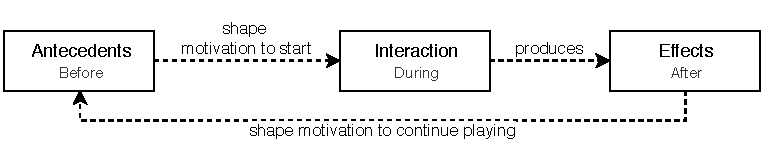
\includegraphics[width=.9\linewidth]{gfx/model/temporalDimension}} \quad
\caption{The Temporal Dimension of  \ac{PX}}\label{fig:temporalDimension}
\end{figure}

The game system is the most concrete layer and corresponds to the technical experience \autocite{Engl2013,Nackea2}. It can be assessed through playability evaluation \autocite{Engl2013,Nacked,Nackea2}. In rehabilitation exergames, it is characterised by the use of non-traditional interaction devices, the support of a rehabilitation goal and the assurance of patients safety. The player layer corresponds to the individual experience of playing a game \autocite{Engl2013,Nackea2} and is assessed through \ac{PX} evaluation \autocite{Engl2013,Nacked,Nackea2,Elson2014}. In rehabilitation exergames, it considers players' health status and progress through their therapies. The context is the most abstract layer. It represents the contextual gameplay experience \autocite{Engl2013} and can be assessed using methods such as sociological studies \autocite{Nacked}. The layers of abstraction are further described in \autoref{sec:layers_abstraction}.

\subsubsection{Relation among dimensions}
\label{sec:rel_among_dimensions}
Each layer of abstraction can be studied throughout those three moments to analyse \ac{PX} as illustrated in \autoref{fig:pxModel} described below.

\begin{figure}[bth]
\myfloatalign
{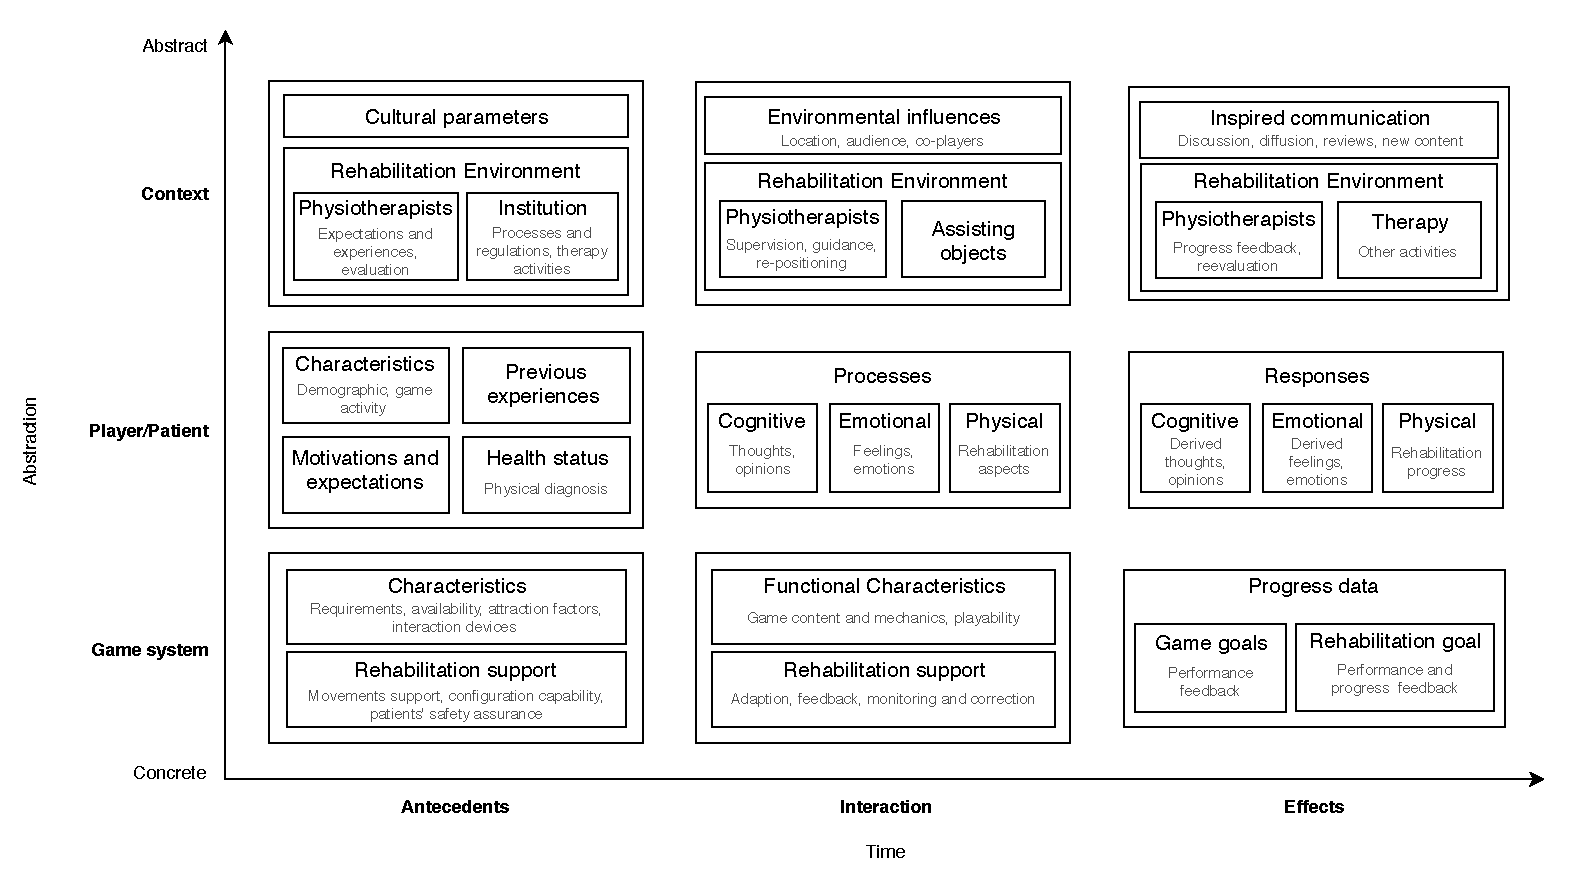
\includegraphics[width=\linewidth]{gfx/model/pxModel}} \quad
\caption{\ac{PX} Layers of Abstraction over Time}\label{fig:pxModel}
\end{figure}

% Antecedents
Antecedents represent everything that occurs before interaction between a player and a game \autocite{Fernandez2008}. Antecedents comprise intrinsic and extrinsic motivators that lead players to start or continue playing a game \autocite{Fernandez2008}. Before interaction, the context is defined by cultural parameters that affect players' opportunity of playing a game \autocite{Elson2014,Nacked}. Cultural parameters include norms, game community, peer groups \autocite{Elson2014,Nacked}. Also, the context comprises the health institution regulations and physiotherapists' expectations, criteria and experience with rehabilitation exergames and technology. Meanwhile, the player is defined by his/her demographics characteristics \autocite{Elson2014,Fernandez2008}, game preferences and habits \autocite{Fernandez2008}, previous experiences \autocite{Nacked,Elson2014}, motivations, expectations (including expectations towards his/her therapy), willingness to use rehabilitation exergames and health diagnosis (i.e., pathology, physical skills, functional independence). On the other hand, the game is defined by its characteristics, availability, attraction factors and marketing \autocite{Elson2014,Nacked}. In the context o physical rehabilitation, it comprises the capability of the game to support a therapeutic goal, be configurable, and ensure patients safety.

% Interaction
Interaction occurs when players actually play or use a digital \autocite{Elson2014,Fernandez2008,Nacked} game motivated by the antecedents \autocite{Fernandez2008}. The interaction moment affects the players' perception of a game depending on their experience \autocite{Fernandez2008}. In rehabilitation exergames, it would also affect physiotherapists' perception. Thus, interaction has a direct relation to future experiences. During the interaction, the context layer comprises different environmental aspects such as location \autocite{Elson2014,Engl2013}, audience, other players \autocite{Elson2014,DeKort2007b,Mayra} and physiotherapists. The player layer comprises the sum of psychological processes and behaviours experienced by players while playing a game \autocite{Elson2014}. That includes \ac{PX} aspects such as enjoyment, presence and flow \autocite{Elson2014}. In the rehabilitation context, it includes physical processes experienced by players that contribute to achieving the expected rehabilitation goal. On the other hand, the game layer comprises the game content, mechanics and functionality \autocite{Elson2014,Engl2013,Nackea2}. In the rehabilitation context, it comprises the games' capability to enable or facilitate players adaption, effective feedback provision, monitoring, exercise correction and physical objects support.

% Effects
The effects are the consequences that result from interaction \autocite{Fernandez2008} and form a feedback loop that affects proceeding interactions \autocite{Nacked,Elson2014}. Effects can be short-term and long-term. Short-term effects are temporary changes in thoughts, feelings and behaviours right after an interaction. Meanwhile, long-term effects are consequences of repeated episodes of interaction \autocite{Elson2014}. After the interaction, the context layer comprises all forms of communication caused or inspired by playing a game \autocite{Elson2014}. The player layer is represented by cognitive and emotional responses derived from an interaction \autocite{Fernandez2008}. In the context of rehabilitation, this layer involves physical responses associated with the expected rehabilitation goal. The game layer comprises the quality of progress data regarding the achievement of the rehabilitation goal.

Additionally, \ac{PX} is affected by time \autocite{Nackea2}. Each layer of abstraction changes over time. The game system changes according to technological steps, which are mainly imposed by consoles manufacturers. The player layer changes gradually based on psychological and physiological processes experienced by players. Finally, the context layer changes based on sociological, economic or political changes that affect players.

% -----------------------------------------------
\section{Discussion} % Discussion %-----------------------------------------------
\label{sec:discussion_model}
%%%%% Reiterate the Research Problem/State the Major Findings:
% Comprehensive model for Rehabilitation exergames
% PX studied in two dimensions: time: before, during, after; level of abstraction: context, player/patient, game system + constraints identified in previous study
% Integrate models to explain relations among layers and dimensions of \a{PX}
Although there are models to study \ac{PX} for game systems, those do not integrate constraints derived from the use of rehabilitation exergames since the models were constructed based on entertainment games. Therefore, we conducted a qualitative study to explore the constructs and concepts of existing \ac{PX} models and integrate them with the rehabilitation constraints that we identified in a previous study (See \autoref{ch:characterising}). The purpose of the study was to design a comprehensive model to study and understand \ac{PX} in rehabilitation exergames. The model is constructed by two dimensions, time and level of abstraction. 

%%%%%%% Explain the Meaning of the Findings and Why They are Important: expected? unexpected? (explain these especially). unusual or unanticipated patterns or trends that emerged from your results and explain their meaning in relation to the research problem.
% PX study as an iterative process, consequences affect -> future antecedents
Regarding the time dimension, \ac{PX} should be studied considering three moments: its antecedents (before), the interaction itself (during) and its effects (after), which is similar to \ac{UX} \autocite{iso9241:210}. As a consequence, studying or evaluating \ac{PX} may represent an iterative process since the effects of a interaction become the antecedents of future experiences.

About abstraction, three levels were identified in the literature, the context, the player and the game system. The context was enriched with rehabilitation environment constraints represented in institutions, physiotherapists and therapy activities.  The player layer was enriched including characteristics of players as patients of rehabilitation therapies.  Finally, the game system was extended with requirements that an exergame should meet to offer an experience in rehabilitation therapies.

% Expected: important role of physios adn insitutions as antecedents to trigger interaction, physios as partipators of interaction and progress feedback (/)
% consider physiotherapists vision (clinical(evaluators) and as users)
As expected, our findings remarked the role of the rehabilitation context at each moment of \ac{PX}. Particularly, it allows identifying when physiotherapists play a role of users (e.g. when configuring a game) or as evaluators (e.g. to validate the quality of progress data). Our final model includes it as part of the context abstraction layer and develops it along the three moments of \ac{PX}. We highlighted the role of physiotherapists and institutions as antecedents that may cause or prevent the use of rehabilitation exergames. To study that, one should consider physiotherapists' expectations, previous experiences and work as evaluators of patients physical status; and health institutions regulations and internal processes. Also, the rehabilitation context may affect the interaction moment. Thus, physiotherapists' role as guide and supervisor and other therapy relates activities should be assessed.  Regarding the effects produced by the rehabilitation context, physiotherapists give feedback, reevaluate and may perform additional therapy activities after an interaction.

Furthermore, the patients' related constraints were reflected in the player layer of abstraction. We renamed this layer to Player/Patient since a rehabilitation exergame player is also a physical therapy patient. In that context, the health status of a patient and his/her expectations towards his/her therapy are antecedents of any interaction. Moreover, physical processes and responses should be considered during and after interaction respectively.

%Understand the role of the Game system in the therapy. And the rehab env. in the game
Regarding the game system layer of abstraction, the model allows to define the characteristics on which  playability should focus on. Additional to the characteristics of entertainment games already defined in literature, we could identify that the capability of an exergame to support a rehabilitation goal, movements and assure patients safety is relevant antecedents. Also, its capability to enable or facilitate adaption to patients, relevant feedback provision, correction and monitoring should be effective during the interaction. Whether it should facilitate or enable those capabilities depends on its degree of autonomy. After the interaction, the quality of feedback about patients' rehabilitation progress should be assessed.

% Important: to study PX considering constraints imposed by rehab. Understand when each constraint play a role.
The mapping between the rehabilitation constraints and the existing \ac{PX} models allow us to understand how rehabilitation exergames comprises a wider range of aspects than entertainment games and when those come to play a role. As discussed above, each moment and layer of abstraction is affected by the rehabilitation constraints. Thus, the model may allow researchers to know when on what to assess when studying rehabilitation exergames depending on the needs that they have.

%%%%% Relate the Findings to Similar Studies: compare your results with other studies or use the studies to support a claim.

%%%% End: concise summary of the principal implications of the findings regardless of significance. Why you believe the findings and conclusions of your study are important and how they support broader knowledge or understanding of the research problem. 

%%%%This can be followed by any recommendations for further research. A more general claim or possible conclusion arising from the results. E.g. new research questions. 
% qualitative, no generalisation
% Number of models included
Our findings are limited since we employed a qualitative study to integrate constraints imposed by the rehabilitation environment and current research on \ac{PX}. The constraints had been identified in a previous study that involved interviews with three physiotherapists. Additionally, although we included 7 models of \ac{PX}, we excluded models that explored particular aspects of \ac{PX} such as immersion, enjoyment or flow which may bring new elements to the model. Thus, the generalisation of our results is yet to be proved.

% Unsupervised exergames, studied -> Context -> home, family, ... Game-system not facilitate but enable support. % Limited to supervised rehab exergames
A part of our model was based on the results of a previous study . Those results are based on the experience of the interviewees as physiotherapists at a local hospital. Their answers were mainly based on the idea of using rehabilitation exergames as part of the therapies they supervise. As a consequence, most of the results from that study apply for supervised rehabilitation exergames. Therefore, we highlighted the importance of supporting monitoring, adaption and correction when using an unsupervised ($4_{th}$ degree of autonomy) rehabilitation exergame. Nevertheless, further research should be conducted to validate or extend our assumptions.

% Apply to rehab exergames? % community in rehab exergames????
Additionally, the validity of some of the identified elements in the context o rehabilitation exergames should be studied. The context layer in the reviewed models comprises game communities as part of the antecedents and effects of \c{PX}. In entertainment games, those communities are promoted by players, are highly active and play a relevant role in \ac{PX}. Nonetheless, those communities could be only academic or promoted by health professionals in rehabilitation exergame. Similarly, rehabilitation exergames marketing and diffusion may also be different from entertainment games. As a result, the role of communities and game market in \ac{PX} and their nature remain open for research.

% Other models, exploring how the other context affects layers of abstraction over time
The employed approach allowed us to extend \ac{PX} models to study rehabilitation exergames comprehensively. A similar strategy may be used to proposed models for other kind of games; e.g., educational games. In that case, constraints of the studied context should be identified and mapped into the abstraction and temporal dimensions of\ac{PX}.

% PX in rehab go beyond entertainment. It has a goal that compromises patients' integrity if not properly met. Dimensions offer a comprehensvie iew of PX If rehabilitation aspects
% use the model study rehab exergames, e.g., evaluating PX, designing, etc. to validate and identify its components and relations
% As based to established a methodology that evaluates PX comprehensively considering both dimensions, what and when evaluated
In summary, \ac{PX} in rehabilitation exergames goes beyond entertainment since those are used in rehabilitation environments that may alter or hinder their use. Additionally, rehabilitation exergames players are also patients, and their wellness cannot be compromised. Therefore, we proposed a comprehensive model to study \ac{PX} in rehabilitation exergames, identifying its dimensions and integrating the constraints imposed by both the rehabilitation and entertainment (motivating) goals of that kind of games. The model can be used for research, design and evaluation purposes. Its extensive used may allow validating its claims and identifying unconsidered elements of \ac{PX}. 

% -----------------------------------------------
\section{Conclusion} % Conclusion %-----------------------------------------------
\label{sec:conclusion_model}

% This chapter mix: literature + previous studies to propose a comprehensive model that ... dimensions, rehab constraints
% Relations among dimensions
This chapter presented a comprehensive model to study \ac{PX} in rehabilitation exergames. The model was built upon current research and the rehabilitation constraints identified in a previous study. The \ac{PX} model comprises two dimensions, abstraction and time. The levels of abstraction are the context, the player/patient and the game system. The temporal dimension includes three moments of \ac{PX}, represented by the interaction, its antecedents and its effects. It maps rehabilitation and entertainment elements into abstraction dimension and over the temporal dimension. Along with the model, the methods to design it and a discussion of its implications were included.